\documentclass[amssymb,twocolumn,pra,10pt,aps]{revtex4-1}
\usepackage{mathptmx,amsmath,tikz}

\begin{document}
\title{Solutions to the 59th William Lowell Putnam Mathematical Competition \\
    Saturday, December 5, 1998}
\author{Manjul Bhargava, Kiran Kedlaya, and Lenny Ng}
\noaffiliation
\maketitle

\begin{itemize}
\item[A--1]
Consider the plane containing both the axis of the cone and two opposite
vertices of the cube's bottom face.  The cross section of the cone and
the cube in this plane consists of a rectangle of sides $s$ and
$s\sqrt{2}$ inscribed in an isosceles triangle of base $2$ and height
$3$, where $s$ is the side-length of the cube.  (The $s\sqrt{2}$ side
of the rectangle lies on the base of the triangle.)  Similar triangles
yield $s/3 = (1-s\sqrt{2}/2)/1$, or $s = (9\sqrt{2} - 6)/7.$

\item[A--2]
First solution:
to fix notation, let $A$ be the area
of region $DEFG$, and $B$ be the area of $DEIH$; further
let $C$ denote the area of sector $ODE$, which only depends on the
arc length of $s$.  If $[XYZ]$ denotes the area of triangle
$[XYZ]$, then we have
$A = C + [OEG] - [ODF]$ and $B = C + [ODH] - [OEI]$.  But
clearly $[OEG] = [OEI]$ and $[ODF] = [ODH]$, and so
$A + B = 2C$.

\begin{center}
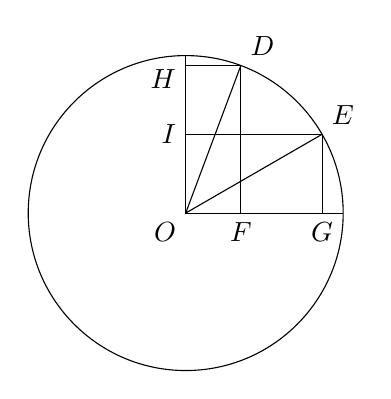
\begin{tikzpicture}
\draw (0,0) circle (2);
\draw (0,2) -- (0,0) -- (2,0);
\draw (1.732,0) -- (1.732,1) -- (0,1);
\draw (.7,0) -- (.7,1.873) -- (0,1.873);
\draw (1.732,1) -- (0,0) -- (.7,1.873);
\draw (0,0) node[anchor=north east] {$O$};
\draw (.7,0) node[anchor=north] {$F$};
\draw (1.732,0) node[anchor=north] {$G$};
\draw (1.732,1) node[anchor=south west] {$E$};
\draw (.7,1.873) node[anchor=south west] {$D$};
\draw (0,1) node[anchor=east] {$I$};
\draw (0,1.7) node[anchor=east] {$H$};
\end{tikzpicture}
\end{center}

Second solution: We may parametrize a point in $s$ by any of
$x$, $y$, or $\theta = \tan^{-1} (y/x)$.  Then $A$ and $B$ are
just the integrals of $y\,dx$ and $x\,dy$ over the appropriate
intervals; thus $A+B$ is the integral of $x\,dy - y\,dx$
(minus because the limits of integration are reversed).
But $d\theta = x\,dy - y\,dx$, and so $A+B = \Delta \theta$
is precisely the radian measure of $s$. (Of course, one can perfectly well
do this problem by computing the two integrals
separately. But what's the fun in that?)

\item[A--3]
If at least one of $f(a)$, $f'(a)$, $f''(a)$, or $f'''(a)$ vanishes
at some point $a$, then we are done.  Hence we may assume each of
$f(x)$, $f'(x)$, $f''(x)$, and $f'''(x)$ is either strictly positive
or strictly negative on the real line.  By replacing $f(x)$ by $-f(x)$
if necessary, we may assume $f''(x)>0$; by replacing $f(x)$
by $f(-x)$ if necessary, we may assume $f'''(x)>0$.  (Notice that these
substitutions do not change the sign of $f(x) f'(x) f''(x) f'''(x)$.)
Now $f''(x)>0$ implies that $f'(x)$ is increasing, and $f'''(x)>0$
implies that $f'(x)$ is convex, so that $f'(x+a)>f'(x)+a f''(x)$
for all $x$ and $a$.  By
letting $a$ increase in the latter inequality, we see that $f'(x+a)$
must be positive for sufficiently large $a$; it follows that
$f'(x)>0$
for all $x$.  Similarly, $f'(x)>0$ and $f''(x)>0$ imply
that $f(x)>0$ for all $x$.  Therefore $f(x) f'(x) f''(x) f'''(x)>0$ for
all $x$, and we are done.

\item[A--4]
The number of digits in the decimal expansion of $A_n$ is the
Fibonacci number $F_n$, where $F_1=1$, $F_2=1$, and $F_n=F_{n-1}
+F_{n-2}$ for $n>2$.  It follows that the sequence $\{A_n\}$, modulo 11,
satisfies the recursion $A_n=(-1)^{F_{n-2}}A_{n-1} + A_{n-2}$.
(Notice that the recursion for $A_n$ depends only on the value of
$F_{n-2}$ modulo 2.)  Using these recursions, we find that
$A_7 \equiv 0$ and $A_8 \equiv 1$ modulo 11, and that
$F_7 \equiv 1$ and $F_8 \equiv 1$ modulo 2.
It follows that $A_n \equiv A_{n+6}$ (mod 11) for all $n\geq 1$.
We find that among
$A_1,A_2,A_3,A_4,A_5$, and $A_6$, only $A_1$ vanishes modulo 11.
Thus 11 divides $A_n$ if and only if $n=6k+1$ for some
nonnegative integer $k$.

\item[A--5]
Define the sequence $D_i$ by the following greedy algorithm:
let $D_1$ be the disc of largest radius (breaking ties arbitrarily),
let $D_2$ be the disc of largest radius not meeting $D_1$, let
$D_3$ be the disc of largest radius not meeting $D_1$ or $D_2$,
and so on, up to some final disc $D_n$.
To see that $E \subseteq \cup_{j=1}^n 3D_j$, consider
a point in $E$; if it lies in one of the $D_i$, we are done. Otherwise,
it lies in a disc $D$ of radius $r$, which meets one of the $D_i$ having
radius $s \geq r$ (this is the only reason a disc can be skipped in
our algorithm). Thus
the centers lie at a distance $t < s+r$, and so every point at distance
less than $r$ from the center of $D$ lies at distance at most
$r + t < 3s$ from the center of the corresponding $D_i$.

\item[A--6]
Recall the inequalities $|AB|^2 + |BC|^2 \geq 2|AB||BC|$ (AM-GM)
and $|AB||BC| \geq 2[ABC]$ (Law of Sines). Also recall that the area of
a triangle with integer coordinates is half an integer
(if its vertices lie at $(0,0), (p,q), (r,s)$, the area is
$|ps-qr|/2$), and that if $A$ and $B$ have integer coordinates, then
$|AB|^2$
is an integer (Pythagoras). Now observe that
\begin{align*}
8[ABC] &\leq |AB|^2+|BC|^2 + 4[ABC] \\
&\leq |AB|^2 + |BC|^2 + 2|AB| |BC| \\
&< 8[ABC]+1,
\end{align*}
and that the first and second expressions are both integers.
We conclude that
$8[ABC] = |AB|^2+ |BC|^2+4[ABC]$, and so $|AB|^2+|BC|^2 =
2|AB| |BC|
= 4[ABC]$; that is, $B$ is a right angle and $AB=BC$, as desired.

\item[B--1]
Notice that
\begin{gather*}
\frac{(x+1/x)^6-(x^6+1/x^6)-2}{(x+1/x)^3+(x^3+1/x^3)} = \\
(x+1/x)^3-(x^3+1/x^3)=3(x+1/x)
\end{gather*}
(difference of squares).  The latter is easily seen
(e.g., by AM-GM) to have minimum value 6
(achieved at $x=1$).

\item[B--2]
Consider a triangle as described by the problem; label its
vertices $A,B,C$ so that $A = (a,b)$, $B$ lies on the $x$-axis,
and $C$ lies on the line $y=x$.  Further let $D = (a,-b)$ be the
reflection of $A$ in the $x$-axis, and let $E = (b,a)$ be
the reflection of $A$ in the line $y=x$.  Then $AB=DB$
and $AC=CE$, and so the perimeter of $ABC$ is
$DB+BC+CE \geq DE = \sqrt{(a-b)^2 + (a+b)^2}
= \sqrt{2a^2+2b^2}$.  It is clear that this lower bound can
be achieved; just set $B$ (resp. $C$) to be the
intersection between the segment $DE$ and the $x$-axis (resp.
line $x=y$); thus the minimum perimeter is in fact
$\sqrt{2a^2+2b^2}$.

\item[B--3]
We use the well-known result that the surface area of the
``sphere cap'' $\{(x,y,z)\,|\,x^2+y^2+z^2=1,\,z\geq z_0\}$ is
simply $2\pi(1-z_0)$.  (This result is easily verified using
calculus; we omit the derivation here.)  Now the desired surface
area is just $2\pi$ minus the surface areas of five identical
halves of sphere caps; these caps, up to isometry, correspond
to $z_0$ being the distance from the center of the pentagon
to any of its sides, i.e., $z_0 = \cos \frac{\pi}{5}$.  Thus
the desired area is
$2\pi - \frac{5}{2} \left(2\pi (1-\cos\frac{\pi}{5})\right)
= 5\pi\cos\frac{\pi}{5} - 3\pi$ (i.e., $B=\pi/2$).

\item[B--4]
For convenience, define $f_{m,n}(i) = \lfloor \frac{i}{m} \rfloor +
\lfloor \frac{i}{n} \rfloor$, so that the given sum is
$S(m,n) = \sum_{i=0}^{mn-1} (-1)^{f_{m,n}(i)}$.
If $m$ and $n$ are both odd, then $S(m,n)$ is the sum of
an odd number of $\pm 1$'s, and thus cannot be zero.  Now consider
the case where $m$ and $n$ have opposite parity.  Note that
$\lfloor \frac{i}{m} \rfloor + \lfloor k - \frac{i+1}{m} \rfloor
= k-1$ for all integers $i,k,m$.  Thus
$\lfloor \frac{i}{m} \rfloor + \lfloor \frac{mn-i-1}{m} \rfloor
= n-1$ and $\lfloor \frac{i}{n} \rfloor + \lfloor \frac{mn-i-1}{n}
\rfloor = m-1$; this implies that $f_{m,n}(i) + f_{m,n}(mn-i-1) =
m+n-2$ is odd, and so $(-1)^{f_{m,n}(i)} =
-(-1)^{f_{m,n}(mn-i-1)}$ for
all $i$.  It follows that $S(m,n) = 0$ if $m$ and
$n$ have opposite parity.

Now suppose that $m=2k$ and $n=2l$ are both even.
Then $\lfloor \frac{2j}{2m} \rfloor = \lfloor \frac{2j+1}{2m} \rfloor$
for all $j$, so $S$ can be computed as twice the sum over only even
indices:
\[
S(2k, 2l) = 2 \sum_{i=0}^{2kl-1} (-1)^{f_{k,l}(i)}
= S(k,l)(1 + (-1)^{k+l}).
\]
Thus $S(2k,2l)$ vanishes if and only if $S(k,l)$ vanishes (if $1 +
(-1)^{k+l} = 0$, then $k$ and $l$ have opposite parity and so
$S(k,l)$ also vanishes).

Piecing our various cases together, we easily deduce that
$S(m,n) = 0$ if and only if the highest powers of 2 dividing
$m$ and $n$ are different.

\item[B--5]
Write $N=(10^{1998}-1)/9$.  Then
\begin{align*}
\sqrt{N} &=\frac{10^{999}}{3}\sqrt{1-10^{-1998}} \\
&=\frac{10^{999}}{3}
(1-\frac{1}{2}10^{-1998} + r),
\end{align*}
where $r<10^{-2000}$.  Now the digits after the decimal point of
$10^{999}/3$ are given by $.3333\ldots$, while
the digits after the decimal point
of $\frac{1}{6}10^{-999}$ are given by $.00000\ldots 1666666\ldots$.
It follows that the first 1000 digits of $\sqrt N$ are given
by $.33333\ldots 3331$;  in particular, the thousandth digit is $1$.

\item[B--6]
First solution: Write $p(n) = n^3 + an^2 + bn + c$. Note that $p(n)$
and $p(n+2)$ have the same parity, and recall that any perfect square
is congruent to 0 or 1 (mod 4). Thus if $p(n)$ and $p(n+2)$ are perfect
squares, they are congruent mod 4. But $p(n+2) - p(n) \equiv 2n^2 + 2b$
(mod 4), which is not divisible by 4 if $n$ and $b$ have opposite parity.
%
% and likewise for $p(n+1)$ and $p(n+3)$.
%But the ``third difference'' of $p$ is $p(n) -
%3p(n+1) + 3p(n+2) - p(n+3) = 6$ (easy calculation), so that $p(n) +
%p(n+1) - p(n+2) - p(n+3) \equiv 2$ (mod 4). Thus not all of $p(n), p(n+1),
%p(n+2), p(n+3)$ can be perfect squares.
%(n+2)^3 + a(n+2)^2 + b(n+2) + c
%n^3 + an^2 + bn + c
%== 2n^2 + 2b

Second solution:
We prove more generally that for any polynomial $P(z)$ with integer
coefficients which is not a perfect square, there exists a positive
integer $n$ such that $P(n)$ is not a perfect square. Of course it
suffices to assume $P(z)$ has no repeated factors, which is to say $P(z)$
and its derivative $P'(z)$ are relatively prime.

In particular, if we carry out the Euclidean algorithm on $P(z)$ and $P'(z)$
without dividing, we get an integer $D$ (the discriminant of $P$) such that
the greatest common divisor of $P(n)$ and $P'(n)$ divides $D$ for any $n$.
Now there exist infinitely many primes $p$ such that $p$ divides $P(n)$ for
some $n$: if there were only finitely many, say, $p_1, \dots, p_k$, then
for any $n$ divisible by $m = P(0) p_1 p_2 \cdots p_k$, we have $P(n)
\equiv P(0) \pmod{m}$, that is, $P(n)/P(0)$ is not divisible by $p_1,
\dots, p_k$, so must be $\pm 1$, but then $P$ takes some value infinitely
many times, contradiction. In particular, we can choose some such $p$ not
dividing $D$, and choose $n$ such that $p$ divides $P(n)$. Then $P(n+kp)
\equiv P(n) + kp P'(n) (\mathrm{mod}\,p)$
(write out the Taylor series of the left side);
in particular, since $p$ does not divide $P'(n)$, we can find some $k$
such that $P(n+kp)$ is divisible by $p$ but not by $p^2$, and so
is not a perfect square.

Third solution: (from David Rusin, David Savitt, and Richard Stanley
independently)
Assume that $n^{3}+an^{2}+bn+c$ is a square for all $n>0$.
For sufficiently large $n$,
\begin{align*}
(n^{3/2} + \frac{1}{2} an^{1/2} - 1)^{2} &< n^{3} + an^{2}+bn+c \\
&<  (n^{3/2}+ \frac{1}{2} an^{1/2}+1)^{2};
\end{align*}
thus if $n$ is a large even perfect square, we have $n^{3}+an^{2}+bn+c =
(n^{3/2} + \frac{1}{2} an^{1/2})^{2}$. We conclude this is an
equality of polynomials, but the right-hand side
is not a perfect square for $n$ an even non-square, contradiction.
(The reader might try generalizing this approach to arbitrary polynomials.
A related argument, due to Greg Kuperberg: write $\sqrt{n^3+an^2+bn+c}$
as $n^{3/2}$ times a power series in $1/n$ and take two finite differences
to get an expression which tends to 0 as $n \to \infty$, contradiction.)

Note: in case $n^3 + an^2 + bn + c$ has no repeated factors, it is a
square for only finitely many $n$, by a theorem of Siegel; work of Baker gives
an explicit (but large) bound on such $n$. (I don't know whether the graders
will accept this as a solution, though.)

\end{itemize}

\end{document}
